\chapter{Diagrammi di interazione e di classe UML}

\section{Verso la progettazione a oggetti}

\qs{}{Come si progetta a oggetti?}

\begin{itemize}
    \item [$\Rightarrow$] \fancyglitter{Codifica}: si progetta mentre
    si codifica;
    \item [$\Rightarrow$] \fancyglitter{Disegno, poi codifica}: si
    disegnano i diagrammi UML e poi si codifica;
    \item [$\Rightarrow$] \fancyglitter{Solo disegno}: si disegnano i
    diagrammi UML e lo strumento genera ogni cosa da essi.
\end{itemize}

\nt{Solitamente si sceglie di disegnare e poi codificare.}

\subsection{Modellazione dinamica e statica}

\dfn{Modelli dinamici}{Rappresentano il comportamento del sistema,
la collaborazione tra oggetti per realizzare dei Casi d'Uso. Di solito
si utilizzano i diagrammi di interazione UML.}

\dfn{Modelli statici}{
    Servono per definire package, nomi delle classi, attributi e
    firme di operazioni. Di solito si utilizzano i diagrammi delle
    classi UML.
}

\nt{Solitamente si creano in parallelo sia i modelli dinamici che
statici.}
\pagebreak
\ex{Modelli statici e dinamici}{
    \begin{center}
        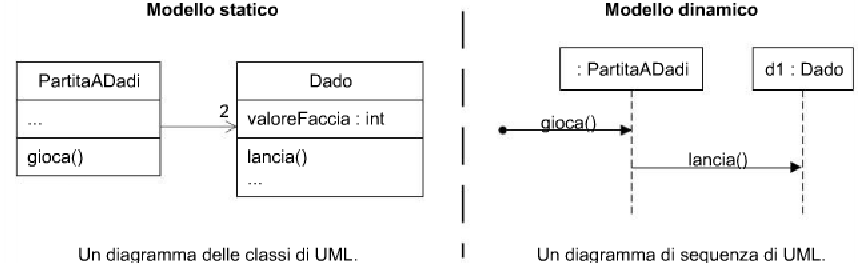
\includegraphics[scale=0.45]{images/Modelli statici e dinamici.png}
    \end{center}
}

\begin{itemize}
    \item [$\Rightarrow$] La maggior parte del lavoro utile e difficile
    avviene nel disegno dei diagrammi di interazione (o di sequenza);
    \item [$\Rightarrow$] Durante la modellazione dinamica si pensa
    a quali oggetti devono esistere e a come collaborano tra loro;
    \item [$\Rightarrow$] Per la modellazione dinamica si fa riferimento
    ai principi GRASP\footnote{Vedi capitolo \ref{GRASP}.}.
\end{itemize}

\subsubsection{Le domande che ci si deve porre sono:}

\begin{itemize}
    \item [$\Rightarrow$] \fancyglitter{Quali} sono le responsabilità
    dell'oggetto?
    \item [$\Rightarrow$] \fancyglitter{Chi} collabora con chi?
    \item [$\Rightarrow$] \fancyglitter{Quali} design pattern devono essere applicati?
\end{itemize}

\subsubsection{La progettazione a oggetti richiede la conoscenza di:}

\begin{itemize}
    \item [$\Rightarrow$] \fancyglitter{Design pattern};
    \item [$\Rightarrow$] \fancyglitter{Principi di assegnazione delle responsabilità}.
\end{itemize}

\section{Diagrammi di interazione}

\dfn{Interazione}{
    Un'\newfancyglitter{interazione} è una specifica di come alcuni
    oggetti si scambiano messaggi nel tempo per eseguire un compito nell'ambito
    di un certo contesto.
}

\nt{Il termine diagramma di interazione si riferisce a due tipi di diagrammi:
\begin{itemize}
    \item [$\Rightarrow$] \fancyglitter{Diagrammi di sequenza};
    \item [$\Rightarrow$] \fancyglitter{Diagrammi di comunicazione}.

\end{itemize}

In questo corso ci concentreremo sui diagrammi di sequenza.
}

\subsubsection{Caratteristiche dei diagrammi di sequenza:}

\begin{itemize}
    \item [$\Rightarrow$] Un'\fancyglitter{interazione} è motivata dalla necessità
    di eseguire un \fancyglitter{compito};
    \item [$\Rightarrow$] Un \fancyglitter{compito} è rappresentato da un 
    \fancyglitter{messaggio} che dà inizio all'interazione (messaggio trovato);
    \item [$\Rightarrow$] Il \fancyglitter{messaggio} è inviato a un oggetto designato
    come \fancyglitter{responsabile} del compito;
    \item [$\Rightarrow$] L'oggetto \fancyglitter{responsabile} collabora con
    altri oggetti (\fancyglitter{partecipanti}) per eseguire il compito;
    \item [$\Rightarrow$] Ciascun \fancyglitter{partecipante} svolge un proprio
    \fancyglitter{ruolo} nell'interazione;
    \item [$\Rightarrow$] La \fancyglitter{collaborazione} avviene mediante 
    \fancyglitter{messaggi} scambiati tra gli oggetti;
    \item [$\Rightarrow$] Ciascun messaggio è una richiesta che un oggetto fa a un altro
    oggetto di eseguire un'\fancyglitter{operazione}.
\end{itemize}

\subsubsection{Vantaggi e svantaggi dei diagrammi di sequenza:}

\begin{itemize}
    \item [\textcolor{green}{\checkmark}] Mostrano chiaramente la sequenza 
    dell'ordinamento temporale dei messaggi.
    \item [\textcolor{red}{\XSolidBrush}] Costringono a estendersi verso destra
    quando si aggiungono nuovi oggetti.
\end{itemize}

\ex{Diagrammi di sequenza}{
    \begin{center}
        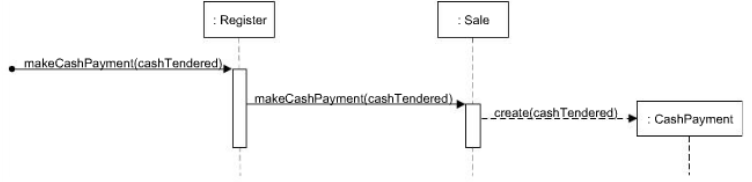
\includegraphics[scale=0.45]{images/Diagramma di sequenza.png}
    \end{center}
}

\subsection{Diagrammi di sequenza del design (DSD)}

\dfn{Design Sequence Diagram (DSD)}{
    Un \newfancyglitter{diagramma di sequenza} di progetto è un diagramma
    di sequenza utilizzato da un punto di vista software o di progetto.
}

\nt{In UP l'insieme di tutti i DSD fa parte del modello di progetto.}

\ex{Notazione di DSD: partecipanti}{
    \begin{center}
        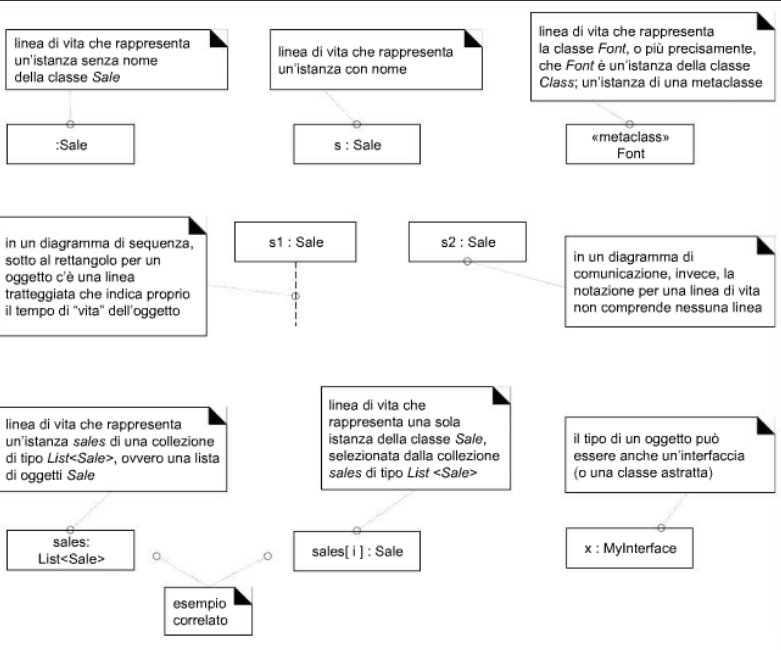
\includegraphics[scale=0.35]{images/Notazione di DSD.png}
    \end{center}
}

\dfn{Singleton}{
    Un \newfancyglitter{singleton} è un pattern nel quale da una classe viene istanziata una sola istanza.
}

\ex{Notazione di DSD: singleton}{
    \begin{center}
        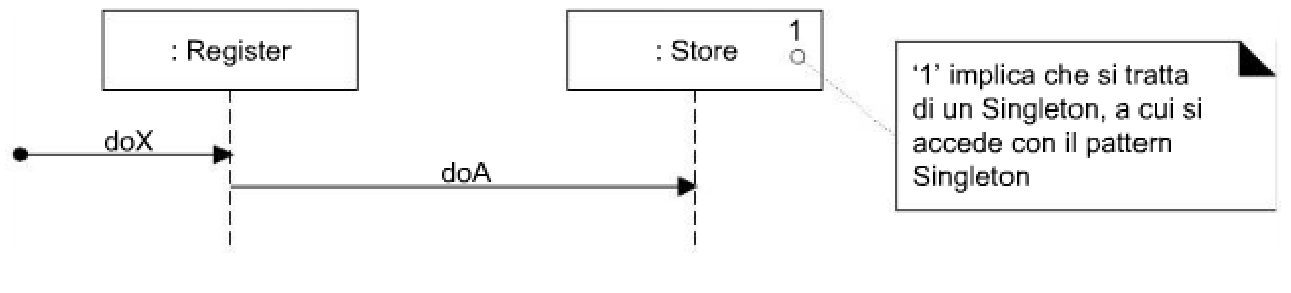
\includegraphics[scale=0.25]{images/Singleton.png}
    \end{center}
}

\ex{Notazione di DSD: messaggi}{
    \begin{center}
        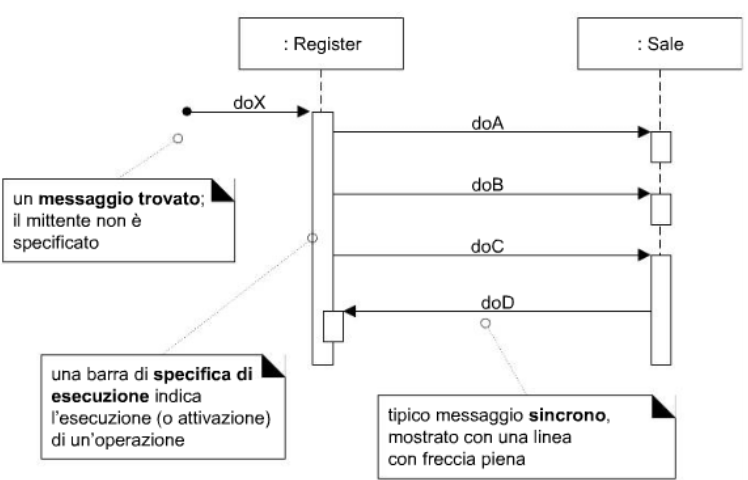
\includegraphics[scale=0.35]{images/Messaggi.png}
    \end{center}
}

\ex{Notazione di DSD: self (this)}{
    \begin{center}
        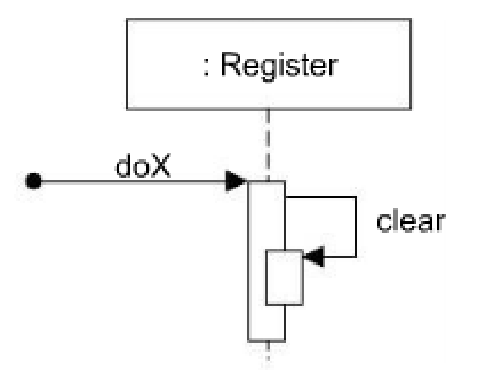
\includegraphics[scale=0.35]{images/Self.png}
    \end{center}
}

\ex{Notazione di DSD: creazione di istanze}{
    \begin{center}
        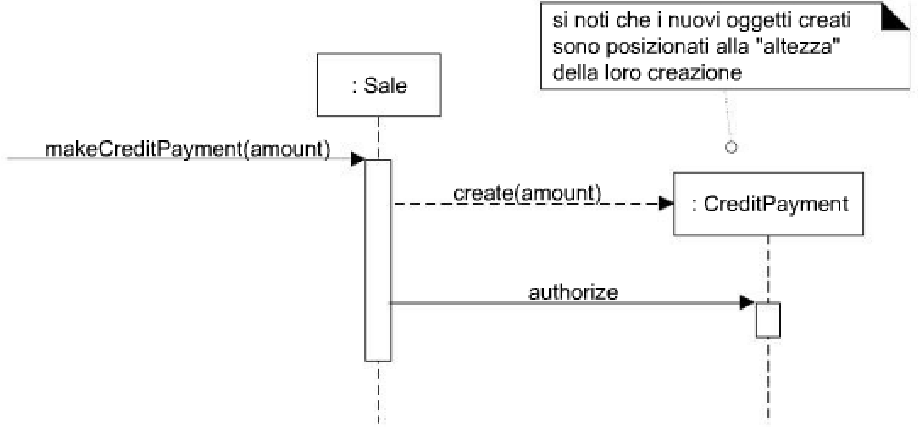
\includegraphics[scale=0.35]{images/Creazione di istanze.png}
    \end{center}
}

\ex{Notazione di DSD: distruzione di oggetti}{
    \begin{center}
        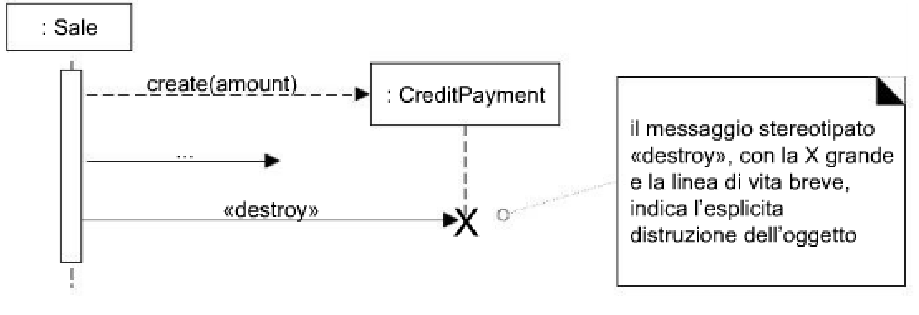
\includegraphics[scale=0.35]{images/Distruzione di oggetti.png}
    \end{center}
}
\pagebreak
\ex{Notazione di DSD: collegamenti}{
    \begin{center}
        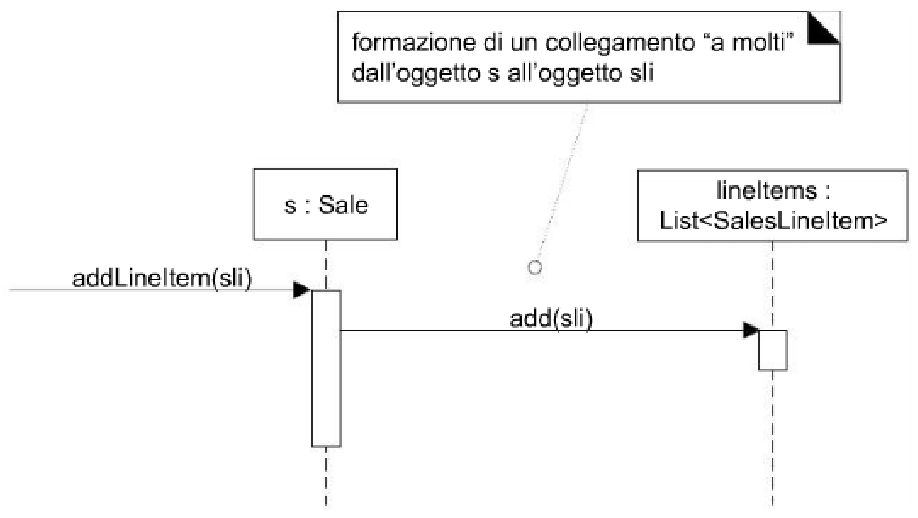
\includegraphics[scale=0.35]{images/Collegamento1.png}
        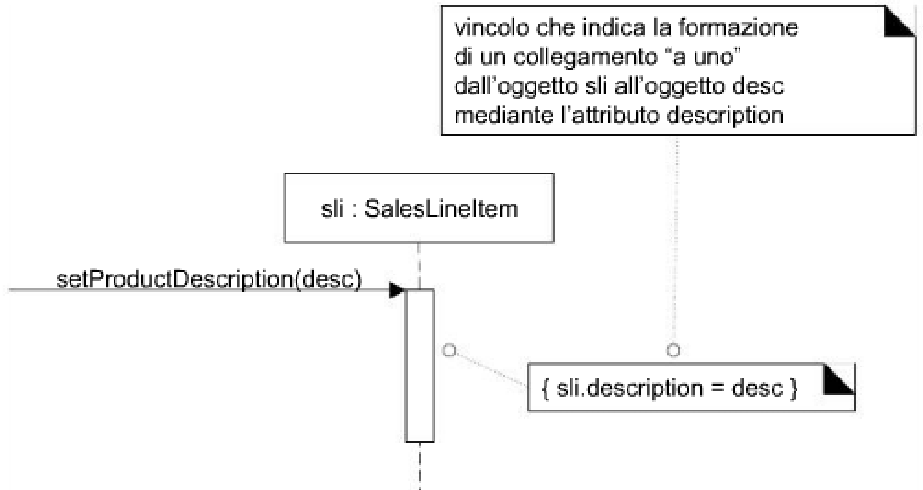
\includegraphics[scale=0.35]{images/Collegamento2.png}
    \end{center}

}

\ex{Notazione di DSD: frame}{
    \begin{center}
        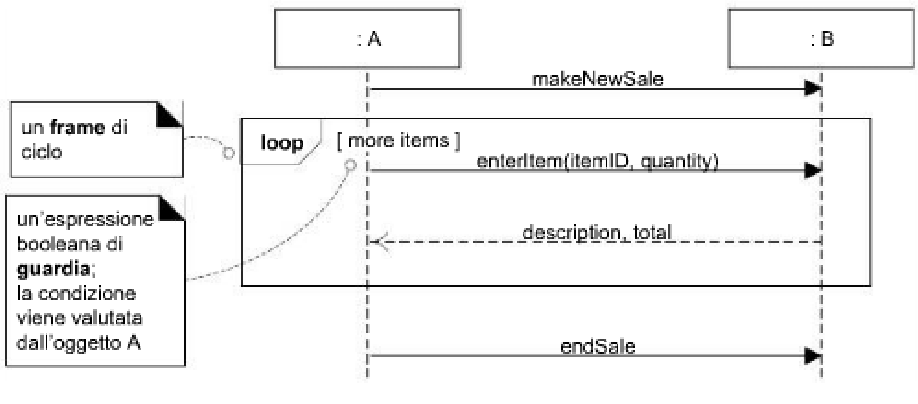
\includegraphics[scale=0.35]{images/Frame.png}
    \end{center}
}
\pagebreak
\ex{Notazione di DSD: condizionale}{
    \begin{center}
        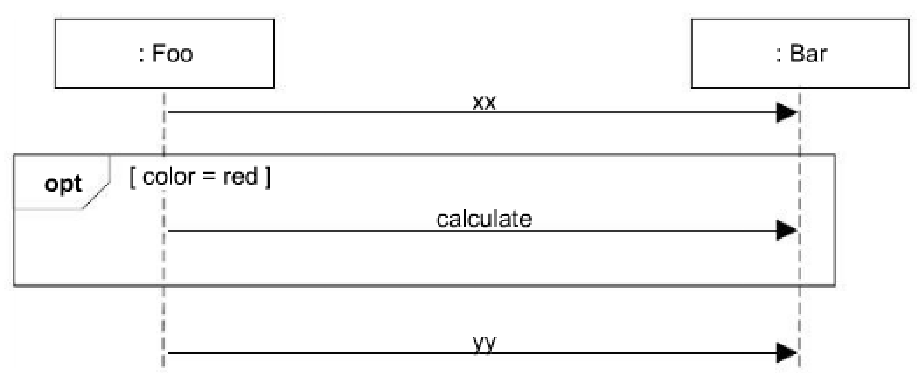
\includegraphics[scale=0.35]{images/Condizioni.png}
    \end{center}
}

\ex{Notazione di DSD: condizionale mutualmente esclusivo}{
    \begin{center}
        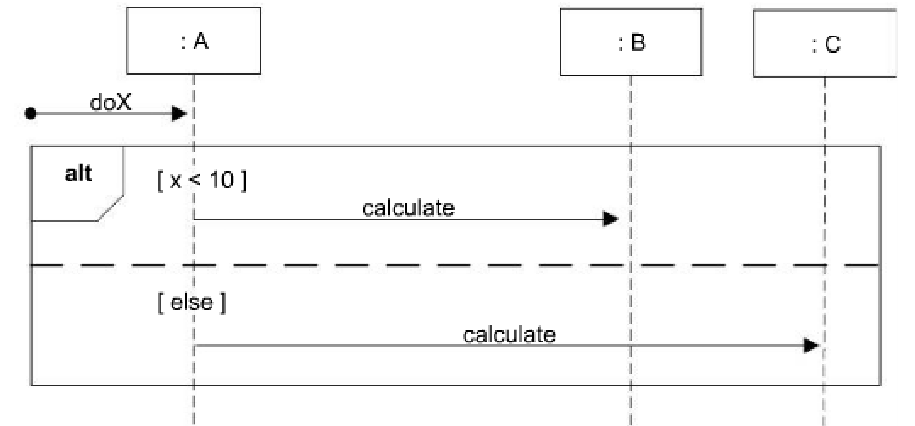
\includegraphics[scale=0.35]{images/Alt.png}
    \end{center}
}

\ex{Notazione di DSD: iterazione su una collezione}{
    \begin{center}
        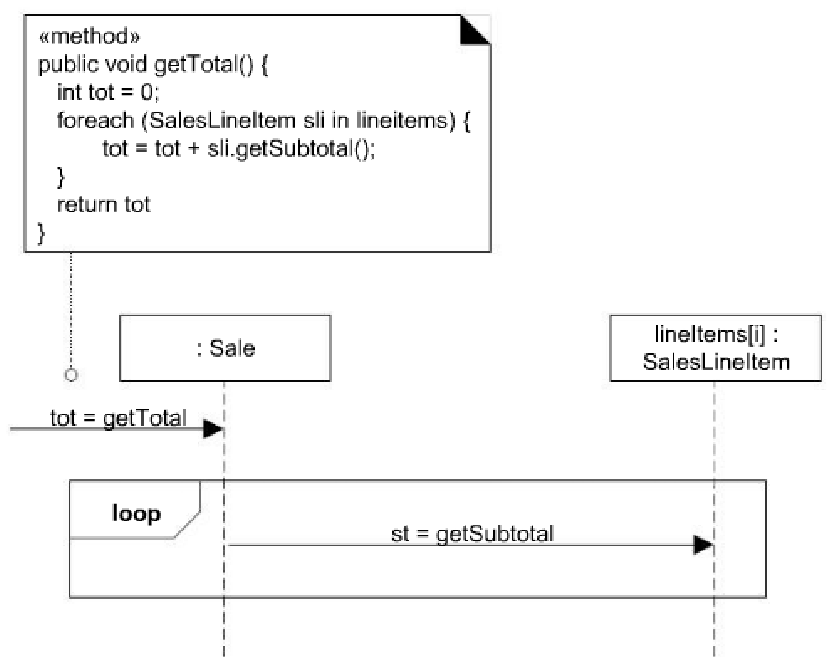
\includegraphics[scale=0.35]{images/Iterazione.png}
    \end{center}
}

\pagebreak

\ex{Notazione di DSD: correlare diagrammi di interazione}{
    \begin{center}
        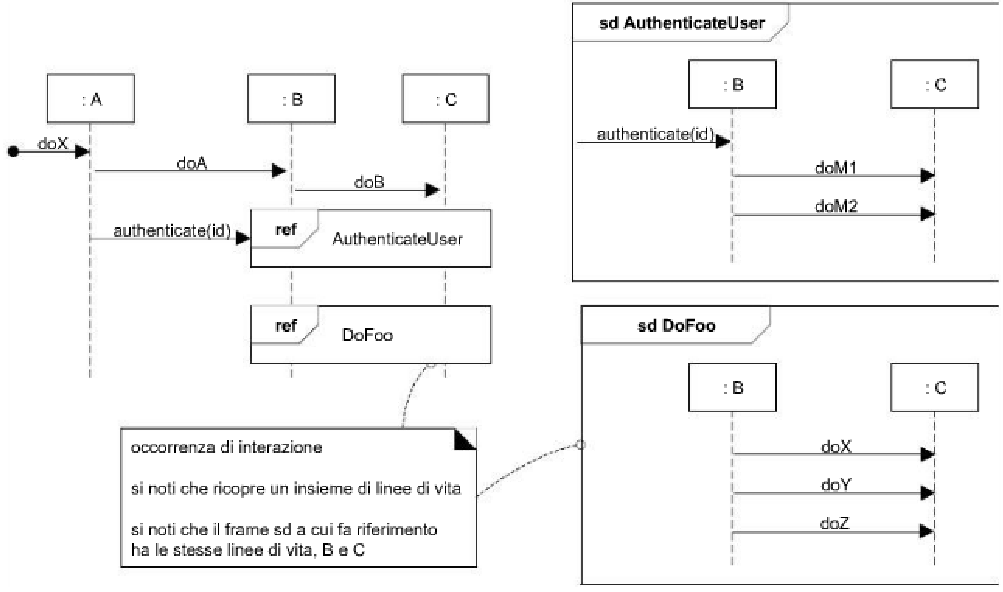
\includegraphics[scale=0.4]{images/Correlare.png}
    \end{center}
}

\ex{Notazione di DSD: invocare metodi statici}{
    \begin{center}
        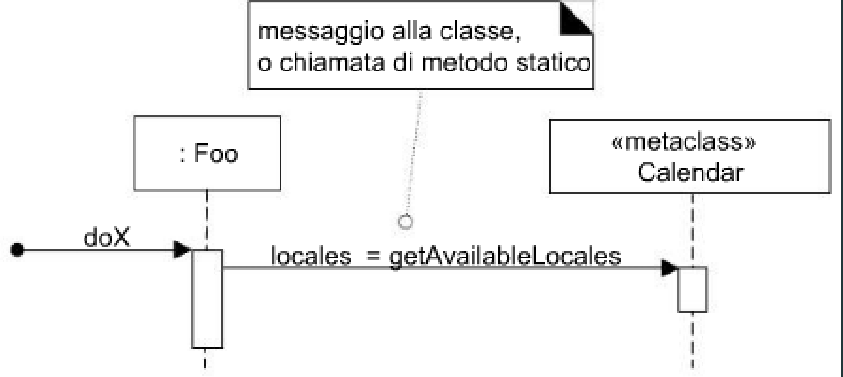
\includegraphics[scale=0.35]{images/Static.png}
    \end{center}
}

\nt{Nel caso di invocazione di metodi statici l'oggetto ricevente è
un'istanza di una meta-classe.}

\pagebreak

\ex{Notazione di DSD: chiamate sincrone e asincrone}{
    \begin{center}
        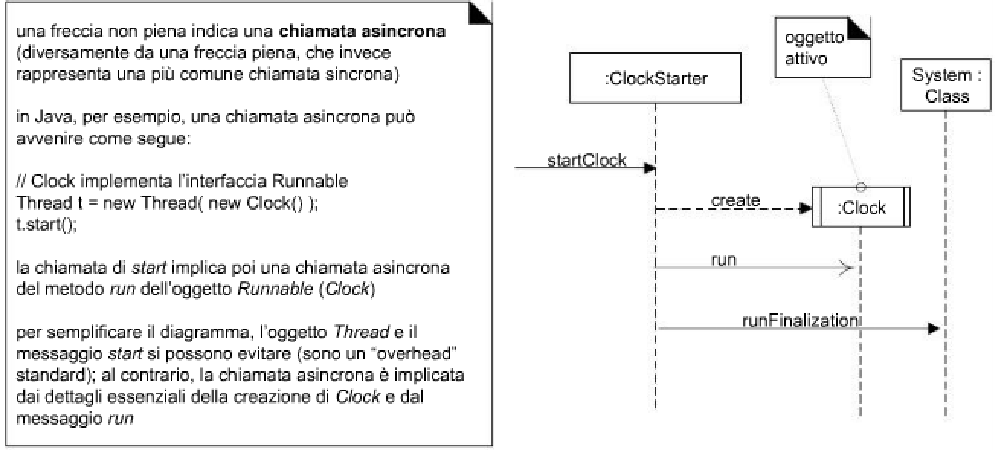
\includegraphics[scale=0.45]{images/Chiamate.png}
    \end{center}
}
\pagebreak
\section{Diagrammi delle classi}

\subsection{Diagrammi di classe del design (DCD)}

\dfn{Design Class Diagram (DCD)}{
    Un \newfancyglitter{diagramma delle classi} di progetto è un diagramma
    delle classi utilizzato da un punto di vista software o di progetto.
}


\nt{In UP l'insieme di tutti i DCD fa parte del modello di progetto.}

\ex{Notazione generale di DCD}{
    \begin{center}
        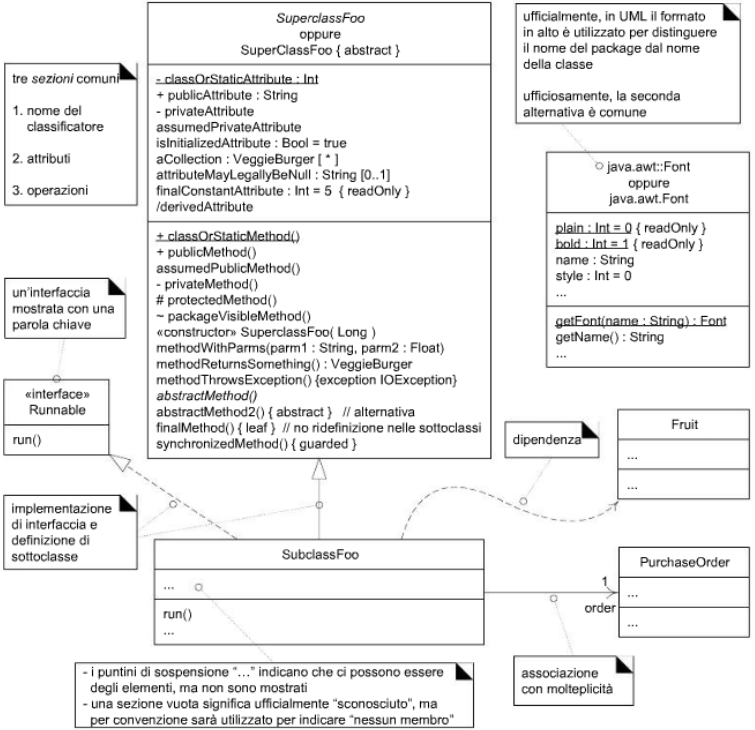
\includegraphics[scale=0.5]{images/Generale.png}
    \end{center}
}

\nt{
    \begin{itemize}
        \item [$\Rightarrow$] \fancyglitter{$+$} indica un attributo pubblico;
        \item [$\Rightarrow$] \fancyglitter{$-$} indica un attributo privato;
        \item [$\Rightarrow$] \fancyglitter{\#} indica un attributo protetto;
        \item [$\Rightarrow$] \fancyglitter{\textasciitilde} indica un attributo package.
    \end{itemize}
}

\ex{Notazione di DCD: attributi}{
    \begin{center}
        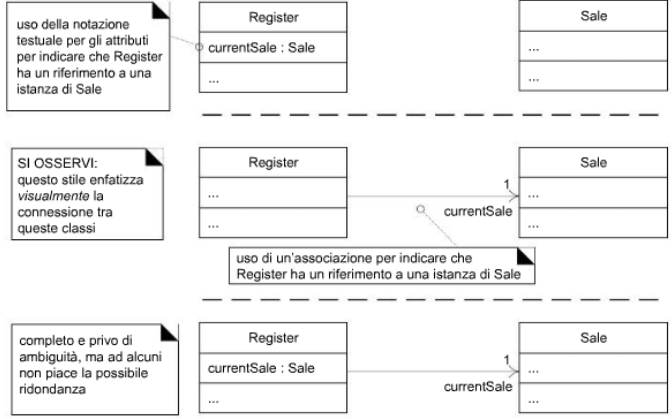
\includegraphics[scale=0.45]{images/Attributi.png}
    \end{center}
}

\nt{Se non viene specificata la visibilità di un attributo si intende
che esso sia privato.}

\ex{Notazione di DCD: parole chiave}{
    \begin{center}
        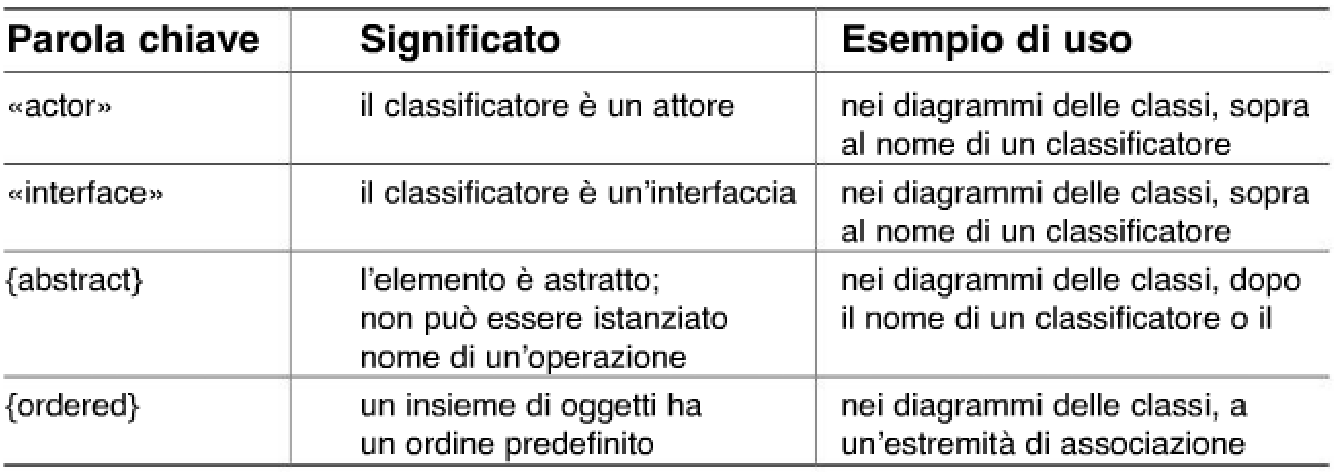
\includegraphics[scale=0.3]{images/Parole chiave.png}
    \end{center}
}
\dfn{Stereotipi}{
    Gli \newfancyglitter{stereotipi} sono un raffinamento di un concetto
    di modellazione esistente.
}

\ex{Notazione di DCD: stereotipi}{
    \begin{center}
        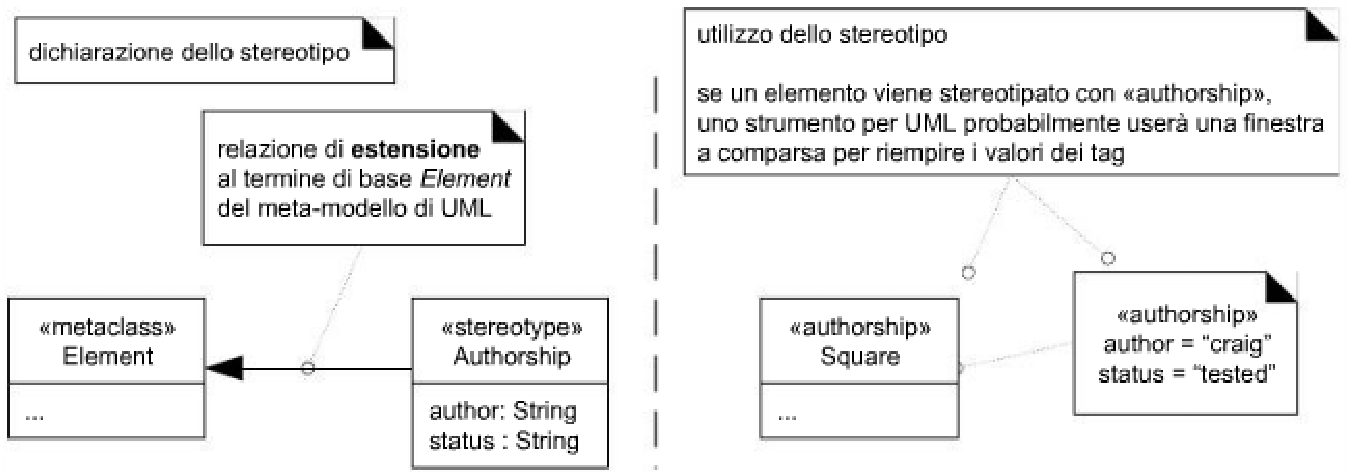
\includegraphics[scale=0.25]{images/Stereotipi.png}
    \end{center}
}

\dfn{Generalizzazione}{
    La \newfancyglitter{generalizzazione} è una relazione tassonomica
    tra una classe più generale e una classe più specifica. Ogni istanza
    della classe specifica è anche un'istanza della classe generale.
}

\nt{La generalizzazione implica \fancyglitter{ereditarietà} nei linguaggi OO.}

\dfn{Linee di dipendenza}{
    Una \newfancyglitter{linea di dipendenza} è una relazione tra due
    classi che indica che un cambiamento nella classe dipendente può
    influenzare la classe dipendente.
}

\ex{Notazione di DCD: dipendenza}{
    \begin{center}
        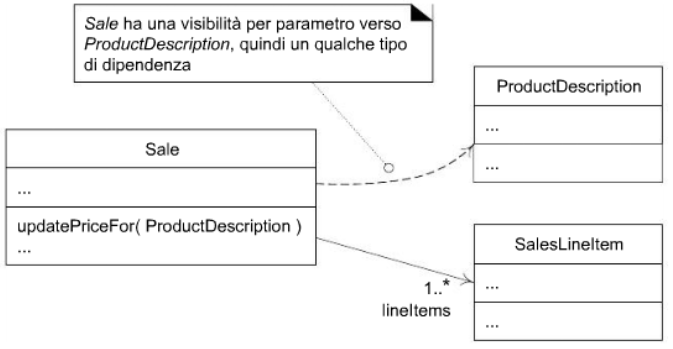
\includegraphics[scale=0.45]{images/Dipendenza.png}
    \end{center}
}

\nt{È importante mantenere un basso accoppiamento tra le classi.}

\subsubsection{Esistono varie tipologie di dipendenze:}

\begin{itemize}
    \item [$\Rightarrow$] Avere un attributo del tipo del fornitore;
    \item [$\Rightarrow$] Inviare un messaggio al fornitore;
    \item [$\Rightarrow$] Ricevere un parametro del tipo del fornitore;
    \item [$\Rightarrow$] Il fornitore è una superclasse o un'interfaccia implementata.
\end{itemize}

\dfn{Interfacce}{
    Un'\newfancyglitter{interfaccia} è un contratto tra un fornitore
    e un cliente. Un cliente può invocare i metodi definiti nell'interfaccia.
    Si hanno due notazioni:
    \begin{itemize}
        \item [$\Rightarrow$] \newfancyglitter{Notazione a pallina} (lollipop),
        indica che una classe X implementa (fornisce) un'interfaccia Y;
        \item [$\Rightarrow$] \newfancyglitter{Notazione a semicerchio} (socket),
        indica che una classe X richiede (usa) un'interfaccia Y.
    \end{itemize}
}
\pagebreak
\ex{Notazione di DCD: composizione}{
    \begin{center}
        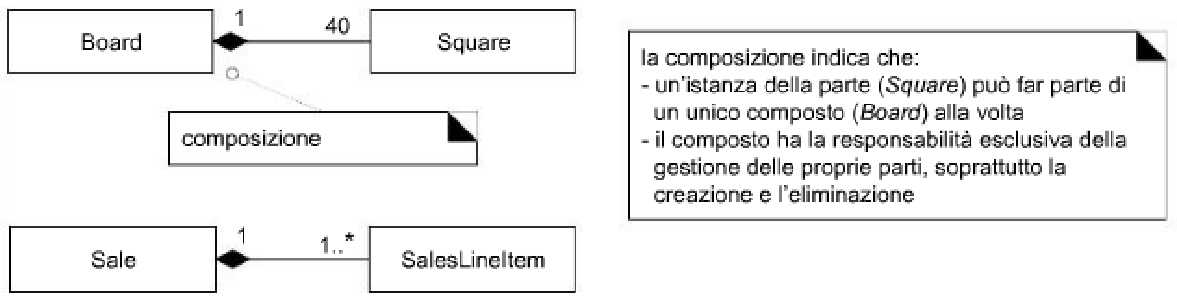
\includegraphics[scale=0.35]{images/Composizione.png}
    \end{center}
}

\ex{Notazione di DCD: singleton}{
    \begin{center}
        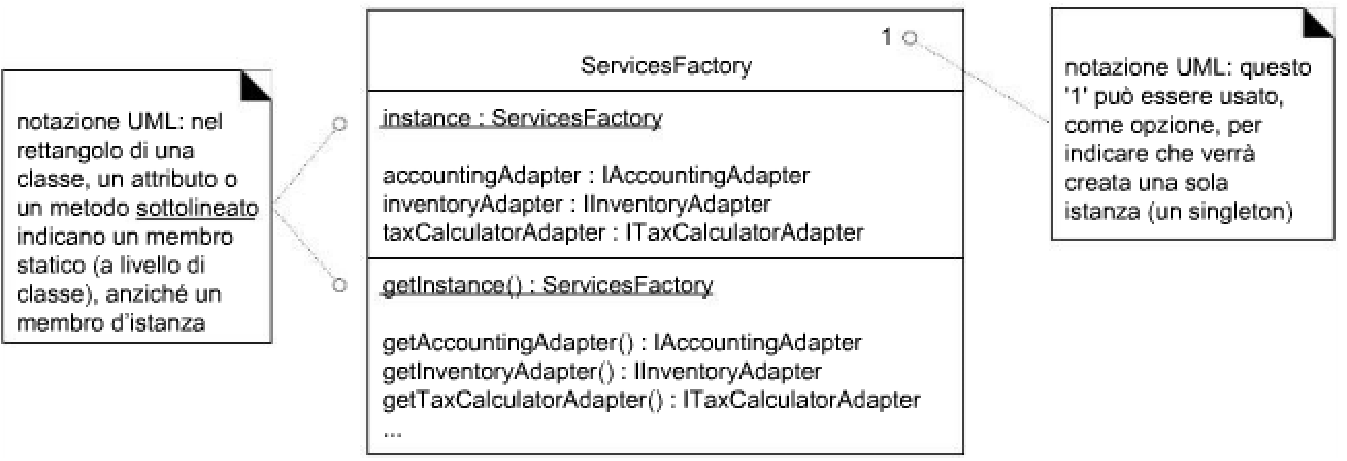
\includegraphics[scale=0.33]{images/Singleton2.png}
    \end{center}
}

\ex{Notazione di DCD: tipi a template}{
    \begin{center}
        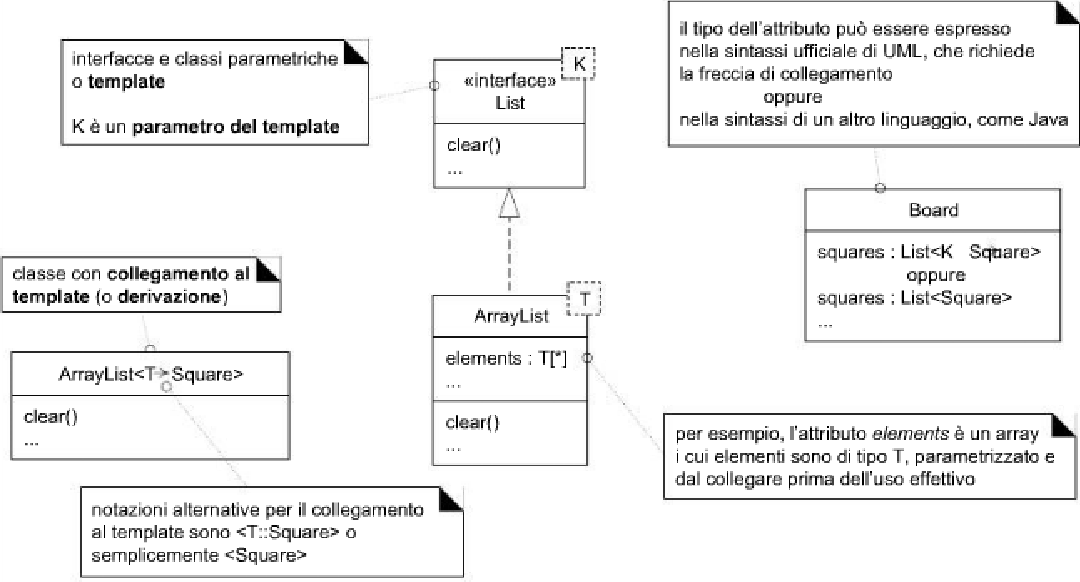
\includegraphics[scale=0.35]{images/Template.png}
    \end{center}
}